\documentclass{class-for-drafts}

\usepackage{hyperref}
%% url
\usepackage{url}
%% maths
\usepackage{amsmath}
%%\usepackage{amsfonts}
\usepackage{amssymb}
%% \usepackage{amsthm}
%% algorithms
%\usepackage{algorithm}
\usepackage{algorithmicx}
%\usepackage[noend]{algpseudocode}
\usepackage[ruled, linesnumbered, noend]{algorithm2e}

%% images
\usepackage{graphicx}
%% inparaenum
\usepackage{paralist}

%% tables
\usepackage{booktabs}
\usepackage{multirow}
%% figures
%\usepackage{caption}
\usepackage{subfig}
%\usepackage[font=small, skip=2pt]{caption}
%\usepackage[font=small]{subfig}
\usepackage{tikz}
\usetikzlibrary{arrows.meta,decorations.pathreplacing,decorations.pathmorphing,plotmarks,shapes,matrix}
\tikzset{>={Latex[width=3pt,length=5pt]}}
%% transform eps in pdf crossplateform
\usepackage{epstopdf}
\usepackage{epsfig}
%% hyphenation
\usepackage{hyphenat}
\hyphenation{brow-sers brow-ser}

\newcommand{\TODO}[1]{\textcolor{red}{#1}}
\newcommand{\REF}[0]{\textcolor{purple}{REF}}

\usepackage{xspace}
\newcommand{\SCAMP}[0]{\textsc{Scamp}\xspace}
\newcommand{\CYCLON}[0]{\textsc{Cyclon}\xspace}
\newcommand{\SPRAY}[0]{\textsc{Spray}\xspace}
\newcommand{\LSEQ}[0]{\textsc{LSeq}\xspace}
\newcommand{\CRATE}[0]{\textsc{Crate}\xspace}
\newcommand{\PEERSIM}[0]{\textsc{PeerSim}\xspace}

\usepackage{amsthm} %% proof env
\newtheorem{definition}{Definition}
\newtheorem{theorem}{Theorem}

%%%%%%%%%%%%%%%%%%%%%%%%%%%%%%%%%%%%%%%%%%%%%%%%%%%%%%%%%%%%%%%%%%%%%%%%%%%%%%%
%%%%%%%%%%%%%%%%%%%%%%%%%%%%%%%%%%%%%%%%%%%%%%%%%%%%%%%%%%%%%%%%%%%%%%%%%%%%%%%
%%%%%%%%%%%%%%%%%%%%%%%%%%%%%%%%%%%%%%%%%%%%%%%%%%%%%%%%%%%%%%%%%%%%%%%%%%%%%%%


\begin{document}

%\title{A better causal broadcast}
\title{Breaking the Scalability Barrier of Causal Broadcast\\for Large
  and Dynamic Networks}

\newcommand{\affLSNN}{L2SN, University of Nantes\\
  2 rue de la Houssini{\`e}re\\
  BP 92208, 44322 Nantes Cedex 3, France\\
  \url{first.last@univ-nantes.fr}}

\author{Brice N{\'e}delec, Pascal Molli, and Achour Most{\'e}faoui \aff \affLSNN}

\proceedings{}

%\copyright{}

\maketitle


\begin{abstract}
  Many distributed protocols and applications rely on causal broadcast to ensure
  consistency.
  %% However, tracking causality while scaling remains an open
  %% problem. 
  However, none of causality tracking state-of-the-art approaches scale in large
  and dynamic networks.   
  %% State-of-the-art approaches do not scale in large and
  %% dynamic networks.
  % State-of-the-art approaches overload messages with control information the
  % size of which increases linearly compared to either the number of processes,
  % or the number of broadcast messages.
  % These approaches are impracticable in large scale systems subject to churn.
  We present a uniform reliable causal broadcast protocol that does not overload
  messages at all while keeping very small local space requirements. We prove
  that it works in both static and dynamic networks.  Now, large and dynamic
  systems can finally afford causal broadcast.
\end{abstract}

\keywords{Uniform, reliable, causal, broadcast.}

%%% Local Variables:
%%% mode: latex
%%% TeX-master: "../paper"
%%% End:


\section{Introduction}


Broadcasting~\cite{hadzilacos1994modular} is a fundamental communication
mechanism for numerous protocols~\cite{shapiro2011comprehensive} and
applications~\cite{nedelec2016crate}. Processes can send messages that will
reach all other processes of their network. In this paper, we focus on causal
broadcast that ensures that processes order message delivery following the
happen before relationship~\cite{lamport1978time}. This aleviates systems from
the burden of tracking causality between its operations. For instance,
distributed collaborative editors perform deletion immediately, for causal
broadcast already guaranteed that the message containing the corresponding
insertion was delivered beforehand.

Unfortunately, causality tracking is
expensive~\cite{charronbost1991concerning}. Current approaches either
\begin{inparaenum}[(i)]
\item piggyback preceding messages in new broadcast
  messages~\cite{birman1987reliable,hadzilacos1993fault},
\item or maintain and send vector clocks along with new broadcast
  messages~\cite{fidge1988timestamps,mattern1989virtual}.
\end{inparaenum}
More recent approaches focus on reducing the size of vectors either by
\begin{inparaenum}[(a)]
\item maintaining local structures to send the least amount of changing data
  (\REF), or by
\item relaxing the causal order using probabilistic
  strucutres~\cite{mostefaoui2017probabilistic}, or by
\item constraining the network topology (\REF).
\end{inparaenum}
None of these approaches scales in large and dynamic networks subject to churn,
for they overload each message with linearly growing data structures that depend
of the number of processes or the number of messages.

In this paper, we solve the scalability issue of causal broadcast. We propose a
uniform reliable broadcast that ensures causal order on message delivery without
any message overhead.  It makes use of FIFO channels (e.g. TCP) and relies on a
peer-sampling protocol~\cite{jelasity2007gossip} ensuring a network without
partitions.  Complexity trade-offs such as the number of messages sent by each
process, or the number of hops before a broadcast message reach all processes,
are independant of our protocol and only depends of the peer-sampling protocol.

The rest of this paper is organized as follows: Section~\ref{sec:preliminaries}
introduces definitions and theorems about causal
broadcast. Section~\ref{sec:proposal} describes our causal broadcast mechanism
and provides the corresponding proofs. Section~\ref{sec:relatedwork} reviews the
related work. We conclude in Section~\ref{sec:conclusion}.


% Broadcast is a communication primitive allowing a process to send a message to
% all other processes in the network. We can add order on message delivery. It
% alleviates the burden of applications to check message relationships. FIFO
% broadcast exists but not so useful. Causal broadcast is very useful; many
% applications require causal order. Holy grail is total order broadcast but not
% scalable, equivalent to consensus.

% We are in point-to-point context.

%%% Local Variables:
%%% mode: latex
%%% TeX-master: "../paper"
%%% End:


\section{Preliminaries}
\label{sec:preliminaries}

Definitions and theorems come from~\cite{hadzilacos1994modular}.

\begin{definition}[Network]
  A network $N$ comprises a set of processes $P$ and a set of edges
  $E: P \times P$. Each process runs a set of instructions
  sequentially. Processes linked by an edge can communicate with each
  other. Processes are faulty if they crash, otherwise they are correct. The set
  of correct processes is $C$. There are no byzantine processes.
\end{definition}

\TODO{Replace ``network'' by  ``distributed system'' ?}


\begin{definition}[Happen before~\cite{lamport1978time}]
  Happen before is a transitive, irreflexive, and antisymmetric relation that
  defines a strict partial orders of events. At process $p$, Event $e$ happens
  before -- or precedes -- Event $e'$ is noted $e_p \rightarrow e'_p$. The
  sending of a message always precedes its receipt: \\
  $\forall p,\,q \in P, s_p(m) \rightarrow r_q(m)$.
\end{definition}

\begin{definition}[Uniform reliable broadcast]
  A process $p$ broadcasts a message $m$ to all processes of the network: \\
  $\forall p \in P,\, (b_p(m) \Leftrightarrow \forall q \in P,\, r_q(m))$. \\
  Uniform reliable broadcast guarantees 3 properties: \\
  \textbf{Validity:} If a correct process broadcasts a message, then it eventually
  delivers it: $\forall p \in C,\, b_p(m) \rightarrow d_p(m)$. \\
  \textbf{Uniform Agreement:} If a process -- correct or not -- delivers a message,
    then all correct processes eventually deliver it:\\
    $\forall p \in P,\, (d_p(m) \implies \forall q \in C,\, d_q(m))$. \\
  \textbf{Uniform Integrity:} A process delivers a message at most once, and
    only if it was previously broadcast:\\
    $\forall p \in P,\, \neg(d_p(m) \rightarrow d_p(m)) \wedge$\\$d_p(m)
    \implies \exists q \in P,\, b_q(m) \rightarrow d_p(m)$.
\end{definition}

\begin{algorithm}[h]
  \SetKwProg{Function}{function}{}{}
\SetKwProg{Upon}{upon}{}{}
\SetKwProg{Initially}{INITIALLY:}{}{}
\SetKwProg{Dissemination}{DISSEMINATION:}{}{}

\small

\DontPrintSemicolon
\LinesNumbered

\Initially {} {
  $Q$ \tcp*{$p$'s neighborhood}
  $received \leftarrow \varnothing$ \tcp*{To detect double receipts}
}

\BlankLine

\Dissemination{}{
  
  \Function{\textsc{R-broadcast}($m$) \tcp*[f]{$b_p(m)$}} { 
    $received \leftarrow received \cup m$ \;
    \lForEach {$q \in Q$} {\textsc{sendTo}($q,\, m$)}
    \textsc{R-deliver}($m$) \tcp*{$d_p(m)$}
  }

  \BlankLine
  
  \Upon{\textsc{receive}($m$)}{
    \If {$m \not \in received$} {
      $received \leftarrow received \cup m$ \;
      \lForEach {$q \in Q$} {\textsc{sendTo}($q,\, m$) \tcp*[f]{forward}}
      \textsc{R-deliver}($m$) \tcp*{$d_p(m)$}
    }
  }
  
}


%%% Local Variables:
%%% mode: latex
%%% TeX-master: "../paper"
%%% End:

  \caption{\label{algo:reliablebroadcast}Uniform reliable broadcast R-broadcast.}
\end{algorithm}

Algorithm~\ref{algo:reliablebroadcast} shows the instructions of a uniform
reliable broadcast. It uses a structure that keeps track of received messages in
order to deliver them at most once. It uses a peer-sampling protocol that
provides neighbors to communicate with, i.e., a set of links. Assuming this
peer-sampling protocol ensures a network without partitions meaning that there
exists at least one path from any process to any correct process, then all
correct processes eventually receive all messages at least once: they either
receive the message directly from the broadcaster or by transitivity. Thus, all
correct processes eventually deliver all messages exactly once. This algorithm
ensures validity, uniform agreement, and uniform integrity.

In addition to reliably conveying messages to all correct processes, broadcast
protocols can ensure that messages are delivered in a specific order.


\begin{definition}[FIFO order]
  If a process broadcasts two messages, processes deliver the first before the
  second:\\
  $\forall p,\,q \in P,\,$\\$b_p(m) \rightarrow b_p(m') \implies d_q(m) \rightarrow
  d_q(m')$.
\end{definition}

\begin{definition}[Local order]
  If a process broadcasts a message after having delivered another message
  broadcast by another process, processes deliver the later before the former:\\
  $\forall p,\,q,\,r,\, \in P,\,p\neq q,\,$\\$b_p(m) \wedge d_q(m) \rightarrow b_q(m') \implies d_r(m) \rightarrow d_r(m')$.
\end{definition}

\begin{definition}[Causal order]
  The delivery order of messages follows the happen before relationships of the
  corresponding broadcasts:\\ $\forall
  p,\,q,\,r \in P,\,$\\$b_p(m) \rightarrow b_q(m') \implies d_r(m) \rightarrow d_r(m')$.
\end{definition}

\begin{theorem}[\label{theo:causal}Causal order equivalence]
  The intersection of FIFO order and Local order is equivalent to Causal order.
\end{theorem}

\begin{figure}
  \begin{center}
  
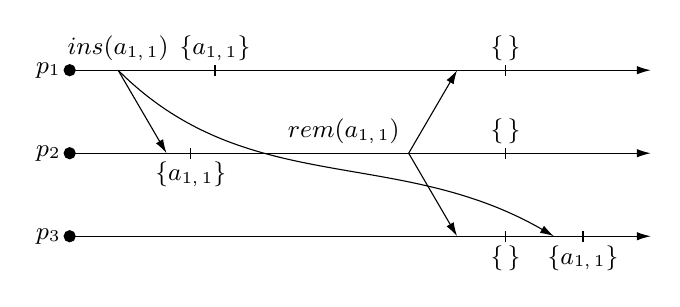
\begin{tikzpicture}[scale=1]
  \small

  \newcommand\X{35pt};
  \newcommand\Y{30pt};
  
  \draw[->](0pt,   0pt)--(6*\X,   0pt);
  \draw[->](0pt, -1*\Y)--(6*\X, -1*\Y);
  \draw[->](0pt, -2*\Y)--(6*\X, -2*\Y);
  
  \draw[fill=black](0pt, 0pt) node[anchor=east]{$p_1$}circle(2pt);
  \draw[fill=black](0pt, -1*\Y) node[anchor=east]{$p_2$}circle(2pt);
  \draw[fill=black](0pt, -2*\Y) node[anchor=east]{$p_3$}circle(2pt);

  \draw[->](0.5 * \X, 0pt)node[anchor=south]{$ins(a_{1,\,1})$}--(1*\X,   -1 * \Y);
%  \draw[->](0.5 * \X, 0pt)-- (2*\X, -1*\Y) -- ( 5 * \X,   -2 * \Y);
  \draw[->](0.5 * \X, 0pt) to[out=-45, in=90+60] ( 5 * \X,   -2 * \Y);
  \draw(1.5*\X, -2pt)--node[anchor=south]{$\{a_{1,\,1} \}$}(1.5*\X, 2pt);
  \draw(1.25 * \X, -2 -1*\Y )--node[anchor=north]{$\{a_{1,\,1} \}$}(1.25 * \X,    2 -1 * \Y);
  \draw(5.3 * \X, -2 -2*\Y )--node[anchor=north]{$\{a_{1,\,1}\}$}(5.3 * \X,   2 -2 * \Y);

  \draw[->](3.5 * \X, -1*\Y )--(4 * \X,   -2 * \Y);
  \draw[->](3.5 * \X, -1*\Y )node[anchor=south east]{$rem(a_{1,\,1})$}--(4 * \X,    0 * \Y);
  \draw(4.5 * \X, -2 -0*\Y )--node[anchor=south]{$\{\,\}$}(4.5 * \X,    2 -0 * \Y);
  \draw(4.5 * \X, -2 -1*\Y )--node[anchor=south]{$\{\,\}$}(4.5 * \X,    2 -1 * \Y);
  \draw(4.5 * \X, -2 -2*\Y )--node[anchor=north]{$\{\,\}$}(4.5 * \X,    2 -2 * \Y);

  % \draw[decorate,decoration={brace,amplitude=6pt,mirror,raise=4pt}]
  % (4.5*\X, -2.5*\Y) -- node[anchor=north, yshift=-10pt]{\small causal order violation = rip consistency} (5.5*\X, -2.5*\Y);
\end{tikzpicture}

%%% Local Variables:
%%% mode: latex
%%% TeX-master: "../paper"
%%% End:

  \caption{\label{fig:generalproblem}Broadcast without causal order
    enforcement.}
  \end{center}
\end{figure}

Figure~\ref{fig:generalproblem} depicts an example where causal order is
violated. Process $p_1$ broadcasts and delivers $m$. Process $p_2$ receives and
delivers $m$. Then, it broadcasts and delivers $m'$. Process $p_3$ receives $m'$
before $m$. Without any causal order enforcement, $p_3$ delivers $m'$ before $m$
violating the condition stating that the delivery of $m$ should precede the
delivery $m'$.

\begin{definition}[Causal broadcast]
  Causal broadcast is a uniform reliable broadcast ensuring causal order.
\end{definition}

Multiple approaches exist to enforce causal order by either piggybacking control
information in each message, or constraining the network topology. In this
paper, we introduce a causal broadcast protocol freed from both these
requirements.


%%% Local Variables:
%%% mode: latex
%%% TeX-master: "../paper"
%%% End:


\section{Causal broadcast for large and dynamic networks}
\label{sec:proposal}

In this section, we introduce a causal broadcast protocol that breaks
scalability barriers for large and dynamic networks. 
% It does not overload
% messages with any control information. 
To provide causal order, most
state-of-the-art~\cite{almeida2008interval,birman1987reliable,fidge1988timestamps,hadzilacos1993fault,mattern1989virtual,mostefaoui2017probabilistic,singhal1992efficient}
approaches are reactive, for they check if message deliveries should be delayed
to avoid causality violations. On the opposite our approach is preventive, for
messages are immediately delivered on receipt without risk of causality
violations. This difference not only removes most of control information
piggybacked in broadcast messages, but also leads to constant delivery
time. Protocols and applications can finally afford causal broadcast in large
and dynamic networks without loss of efficiency.

% This section states  the definitions. It describes our algorithm. It proves that
% it handles both static and dynamic networks. It analyses its complexity.

\subsection{Model}

Definitions and theorems come from~\cite{hadzilacos1994modular}. A network
comprise processes. Processes can communicate with part of the network via
messages. They may not have full knowledge of network membership, for
maintenance costs become too expansive in large and dynamic networks. Instead,
processes build overlay networks with local partial view the size of which is
generally much smaller than the actual network size.

\begin{definition}[Overlay network]
  Just as a network, an overlay network $N$ comprises a set of processes
  $P$. Each Process runs a
  set of instructions sequentially. \\
  An overlay network $N$ also comprises a set of links $E: P \times P$. $p$'s
  neighborhood $Q$ is the set of links departing from $p$. Processes can
  communicate with their neighbors using messages. \\
  Processes are faulty if they crash, otherwise they are correct. The set of
  correct processes is $C$. There are no byzantine processes.
\end{definition}

For the rest of this paper, we will speak of networks and overlay networks
indifferently.

\begin{definition}[Static and dynamic networks]
  A network is static if both its set of processes and its set of edges are
  immutable. Otherwise, the network is dynamic.
\end{definition}

For the rest of the paper, we only consider networks without partitions.

\begin{definition}[Network partition]
  A network has partitions if there exist two correct processes without any path
  between them, i.e., without a link or a sequence of links comprising correct
  processes only.
\end{definition}

%\TODO{Replace ``network'' by  ``distributed system'' ?}

We define time in a logical sense using Lamport's
definition~\cite{lamport1978time}.

\begin{definition}[Happen before]
  Happen before is a transitive, irreflexive, and antisymmetric relation that
  defines a strict partial orders of events. At process $p$, Event $e$ happens
  before -- or precedes -- Event $e'$ is noted $e_p \rightarrow e'_p$. The
  sending of a message $s_p(m)$ always precedes its receipt $r_q(m)$: \\
  $\forall p,\,q \in P, s_p(m) \rightarrow r_q(m)$.
\end{definition}

Processes communicate by sending messages to other processes. They can send
messages to specific processes or all of them.

\begin{definition}[Uniform reliable broadcast]
  A process $p$ can broadcast a message $b_p(m)$, receive a message $r_p(m)$,
  and deliver a message $d_p(m)$.  When a process $p$ broadcasts a message $m$
  to all processes of the network, correct processes eventually receive it: 
  $\forall p \in P,\, (b_p(m) \Leftrightarrow \forall q \in P,\, r_q(m))$. \\
  Uniform reliable broadcast guarantees 3 properties: \\
  \textbf{Validity:} If a correct process broadcasts a message, then it
  eventually
  delivers it: $\forall p \in C,\, b_p(m) \rightarrow d_p(m)$. \\
  \textbf{Uniform Agreement:} If a process -- correct or not -- delivers a
  message,
  then all correct processes eventually deliver it:\\
  $\forall p \in P,\, (d_p(m) \implies \forall q \in C,\, d_q(m))$. \\
  \textbf{Uniform Integrity:} A process delivers a message at most once, and
  only if it was previously broadcast:\\
  $\forall p \in P,\, \neg(d_p(m) \rightarrow d_p(m)) \wedge$\\$d_p(m) \implies
  \exists q \in P,\, b_q(m) \rightarrow d_p(m)$.
\end{definition}

\begin{algorithm}[h]
  \SetKwProg{Function}{function}{}{}
\SetKwProg{Upon}{upon}{}{}
\SetKwProg{Initially}{INITIALLY:}{}{}
\SetKwProg{Dissemination}{DISSEMINATION:}{}{}

\small

\DontPrintSemicolon
\LinesNumbered

\Initially {} {
  $Q$ \tcp*{$p$'s neighborhood}
  $received \leftarrow \varnothing$ \tcp*{To detect double receipts}
}

\BlankLine

\Dissemination{}{
  
  \Function{\textsc{R-broadcast}($m$) \tcp*[f]{$b_p(m)$}} { 
    $received \leftarrow received \cup m$ \;
    \lForEach {$q \in Q$} {\textsc{sendTo}($q,\, m$)}
    \textsc{R-deliver}($m$) \tcp*{$d_p(m)$}
  }

  \BlankLine
  
  \Upon{\textsc{receive}($m$)}{
    \If {$m \not \in received$} {
      $received \leftarrow received \cup m$ \;
      \lForEach {$q \in Q$} {\textsc{sendTo}($q,\, m$) \tcp*[f]{forward}}
      \textsc{R-deliver}($m$) \tcp*{$d_p(m)$}
    }
  }
  
}


%%% Local Variables:
%%% mode: latex
%%% TeX-master: "../paper"
%%% End:

  \caption{\label{algo:reliablebroadcast}R-broadcast at Process $p$.}
\end{algorithm}

Algorithm~\ref{algo:reliablebroadcast} shows the instructions of a uniform
reliable broadcast. It uses a structure that keeps track of received messages in
order to deliver them at most once. 
%It uses a peer-sampling protocol that
%provides neighbors to communicate with, i.e., a set of links. 
%%Assuming a network without partitions meaning that there exists at least one
%path from any process to any correct process, then all correct processes
%eventually receive all messages at least once:
Since processes may not have full membership knowledge, processes must forward
broadcast messages. Since the network does not have partitions, processes either
receive the message directly from the broadcaster or transitively. Thus, all
correct processes eventually deliver all messages exactly once. This algorithm
ensures validity, uniform agreement, and uniform integrity.

In addition to reliably conveying messages to all correct processes, broadcast
protocols can ensure that messages are delivered in a specific order.

To order messages broadcast from one process, we define FIFO order.

\begin{definition}[FIFO order]
  If a process broadcasts two messages, processes deliver the first before the
  second:\\
  $\forall p,\,q \in P,\,$\\$b_p(m) \rightarrow b_p(m') \implies d_q(m) \rightarrow
  d_q(m')$.
\end{definition}

To order messages broadcast by different processes, we define local order.

\begin{definition}[Local order]
  If a process broadcasts a message after having delivered another message
  broadcast by another process, processes deliver the later before the former:\\
  $\forall p,\,q,\,r,\, \in P,\,p\neq q,\,$\\$b_p(m) \wedge d_q(m) \rightarrow b_q(m') \implies d_r(m) \rightarrow d_r(m')$.
\end{definition}

To order messages broadcast by every processes, we define causal order.

\begin{definition}[Causal order]
  The delivery order of messages follows the happen before relationships of the
  corresponding broadcasts:\\ $\forall
  p,\,q,\,r \in P,\,$\\$b_p(m) \rightarrow b_q(m') \implies d_r(m) \rightarrow d_r(m')$.
\end{definition}

\begin{theorem}[\label{theo:causal}Causal order equivalence]
  FIFO order and local order is equivalent to causal order.
\end{theorem}

\begin{definition}[Causal broadcast]
  Causal broadcast is a uniform reliable broadcast ensuring causal order.
\end{definition}

\subsection{Operation}

\begin{algorithm}[h]
  
\SetKwProg{Function}{function}{}{}
\SetKwProg{Upon}{upon}{}{}
\SetKwProg{Initially}{INITIALLY:}{}{}
\SetKwProg{Dissemination}{DISSEMINATION:}{}{}
\SetKwProg{Safety}{SAFETY:}{}{}

\small

\DontPrintSemicolon
\LinesNumbered

\Initially {} {
  $Q$ \tcp*{$p$'s neighborhood, FIFO channels}
  $B \leftarrow \varnothing$ \tcp*{Buffers of messages}
}

\BlankLine

\Safety {} {
  \Upon{\textsc{open}($q$)} {
    \If{$|Q|>1$} {
      $Q \leftarrow Q \setminus q$ \;
      $B[q] \leftarrow \varnothing$ \;
      $\textsc{sendLocked}(p,\, q)$ \;
    }
  }
  
  \BlankLine
  
  \Upon{\textsc{receiveLocked}($from, \, to$) \tcp*[f]{$to=p$}} {
    $\textsc{sendAck}(from,\, to)$ \;
  }
  
  \BlankLine

  \Upon{\textsc{receiveAck}($from,\, to$) \tcp*[f]{$from=p$}} {
    \If {$to \in B$} {
      \lForEach {$m \in B[to]$} {$\textsc{sendTo}(to,\, m)$}
      $B \leftarrow B \setminus to$ \;
      $Q \leftarrow Q \cup to$ \;
    }
  }

  \BlankLine

  \Upon{\textsc{close}($q$)} {
    $B \leftarrow B \setminus q$ \;
  }

}

\BlankLine

\Dissemination {} {

  \Function{\textsc{FBC-broadcast}$^+$($m$) \tcp*[f]{$b_p(m)$}} {    
    \lForEach {$q \in B$} {$B[q] \leftarrow B[q] \cup m$ \tcp*[f]{Buffers}}
    $\textsc{R-broadcast}(m)$ \;
  }
  
  \BlankLine
  
  \Upon{\textsc{R-deliver}($m$)} {
    \lForEach {$q \in B$} {$B[q] \leftarrow B[q] \cup m$ \tcp*[f]{Buffers}}
    $\textsc{FBC-deliver}^+(m)$ \tcp*{$d_p(m)$}
  }

}


%%% Local Variables:
%%% mode: latex
%%% TeX-master: "../paper"
%%% End:

  \caption{\label{algo:bufferbroadcast}\CBROADCAST at Process $p$.}
\end{algorithm}

\begin{figure*}
  \begin{center}
    \subfloat[Part A][\label{fig:preventivesolveA}Process~A broadcasts $a$.]
    {
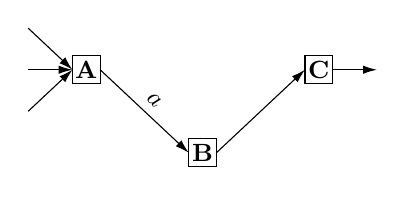
\begin{tikzpicture}[scale=1]
  
  \small
  
  \newcommand\X{210/5pt};
  \newcommand\Y{30pt};
  
  \draw[->] ( -0.5*\X, 0.5*\Y) -- ( -5+0*\X, 0*\Y);
  \draw[->] ( -0.5*\X, 0*\Y) -- ( -5+0*\X, 0*\Y);
  \draw[->] ( -0.5*\X, -0.5*\Y) -- ( -5+0*\X, 0*\Y);  

  \draw[fill=white] (0*\X, 0*\Y) node{\textbf{A}} +(-5pt, -5pt) rectangle +(5pt, 5pt);
  \draw[fill=white] (1*\X, -1*\Y) node{\textbf{B}} +(-5pt, -5pt) rectangle +(5pt, 5pt);
  \draw[fill=white] (2*\X,  0*\Y) node{\textbf{C}} +(-5pt, -5pt) rectangle +(5pt, 5pt);

  \draw[->](5+0*\X, 0*\Y) -- node[sloped, above]{$a$} (-5+1*\X, -1*\Y); %% A->B
  \draw[->](5+1*\X, -1*\Y) -- (-5+2*\X, 0*\Y); %% B->D

  \draw[->](5+2*\X, 0*\Y) -- ( 2.5*\X, 0*\Y);
\end{tikzpicture}}
    \hspace{20pt}
    \subfloat[Part B][\label{fig:preventivesolveB}Process~A wants
    to add a link to Process~D. 
    It sends a locked message $\ell$ to Process~D using one of its FIFO links.]
    {
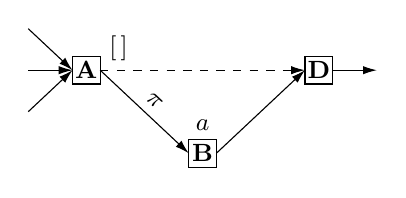
\begin{tikzpicture}[scale=1]
  
  \small
  
  \newcommand\X{210/5pt};
  \newcommand\Y{30pt};
  
  \draw[->] ( -0.5*\X, 0.5*\Y) -- ( -5+0*\X, 0*\Y);
  \draw[->] ( -0.5*\X, 0*\Y) -- ( -5+0*\X, 0*\Y);
  \draw[->] ( -0.5*\X, -0.5*\Y) -- ( -5+0*\X, 0*\Y);  

  \draw[fill=white] (0*\X, 0*\Y) node{\textbf{A}} +(-5pt, -5pt) rectangle +(5pt, 5pt);
  \draw[fill=white] (1*\X, -1*\Y) node{\textbf{B}} +(-5pt, -5pt) rectangle +(5pt, 5pt);
  \draw (1*\X, 5-1*\Y) node[anchor=south]{$a$};
  \draw[fill=white] (2*\X,  0*\Y) node{\textbf{D}} +(-5pt, -5pt) rectangle +(5pt, 5pt);

  \draw[->](5+0*\X, 0*\Y) -- node[sloped, above]{$\pi$} (-5+1*\X, -1*\Y); %% A->B
  \draw[->](5+1*\X, -1*\Y) -- (-5+2*\X, 0*\Y); %% B->D
  
  \draw[->, dashed] (5+0*\X, 0*\Y) node[anchor=south west]{$[\,]$} -- (-5+2*\X, 0*\Y); %% A->B

  \draw[->](5+2*\X, 0*\Y) -- ( 2.5*\X, 0*\Y);
\end{tikzpicture}}
    \hspace{20pt}
    \subfloat[Part C][\label{fig:preventivesolveC}Process~A broadcasts $a'$.
    It does not send it through the new link but buffers it.]
    {
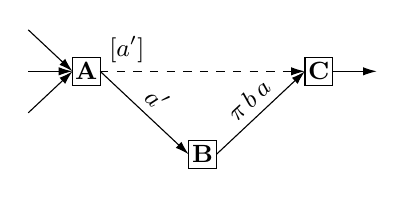
\begin{tikzpicture}[scale=1]
  
  \small
  
  \newcommand\X{210/5pt};
  \newcommand\Y{30pt};
  
  \draw[->] ( -0.5*\X, 0.5*\Y) -- ( -5+0*\X, 0*\Y);
  \draw[->] ( -0.5*\X, 0*\Y) -- ( -5+0*\X, 0*\Y);
  \draw[->] ( -0.5*\X, -0.5*\Y) -- ( -5+0*\X, 0*\Y);  

  \draw[fill=white] (0*\X, 0*\Y) node{\textbf{A}} +(-5pt, -5pt) rectangle +(5pt, 5pt);
  \draw[fill=white] (1*\X, -1*\Y) node{\textbf{B}} +(-5pt, -5pt) rectangle +(5pt, 5pt);
%  \draw (1*\X, 5-1*\Y) node[anchor=south]{$a$};
  \draw[fill=white] (2*\X,  0*\Y) node{\textbf{C}} +(-5pt, -5pt) rectangle +(5pt, 5pt);

  \draw[->](5+0*\X, 0*\Y) -- node[sloped, above]{$a'$} (-5+1*\X, -1*\Y); %% A->B
  \draw[->](5+1*\X, -1*\Y) -- node[sloped, above]{$\pi\,b\,a$} (-5+2*\X, 0*\Y); %% B->D
  
  \draw[->, dashed] (5+0*\X, 0*\Y) node[anchor=south west]{$[a']$} --  (-5+2*\X, 0*\Y); %% A->B

  \draw[->](5+2*\X, 0*\Y) -- ( 2.5*\X, 0*\Y);
\end{tikzpicture}}
    \hspace{20pt}
    \subfloat[Part D][\label{fig:preventivesolveD}Process~D receives
    $\ell$ and acknowledges it to $A$.
    The acknowledgment message $\alpha$ can travel by any communication
    mean.]
    {
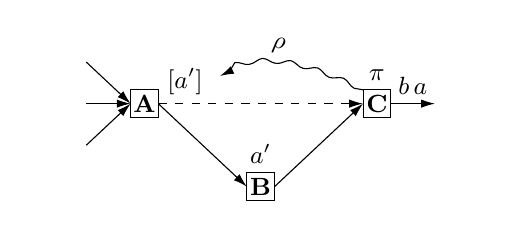
\begin{tikzpicture}[scale=1]
  
  \small
  
  \newcommand\X{210/5pt};
  \newcommand\Y{30pt};

  \draw (-1*\X, 0*\Y);
  \draw (3*\X, 0*\Y);

  
  \draw[->] ( -0.5*\X, 0.5*\Y) -- ( -5+0*\X, 0*\Y);
  \draw[->] ( -0.5*\X, 0*\Y) -- ( -5+0*\X, 0*\Y);
  \draw[->] ( -0.5*\X, -0.5*\Y) -- ( -5+0*\X, 0*\Y);  

  \draw[fill=white] (0*\X, 0*\Y) node{\textbf{A}} +(-5pt, -5pt) rectangle +(5pt, 5pt);
  \draw[fill=white] (1*\X, -1*\Y) node{\textbf{B}} +(-5pt, -5pt) rectangle +(5pt, 5pt);
  \draw (1*\X, 5-1*\Y) node[anchor=south]{$a'$};
  \draw[fill=white] (2*\X,  0*\Y) node{\textbf{C}} +(-5pt, -5pt) rectangle +(5pt, 5pt);
  \draw (2*\X, 5-0*\Y) node[anchor=south]{$\pi$};

  \draw[->](5+0*\X, 0*\Y) -- (-5+1*\X, -1*\Y); %% A->B
  \draw[->](5+1*\X, -1*\Y) -- (-5+2*\X, 0*\Y); %% B->D
  
  \draw[->, dashed] (5+0*\X, 0*\Y) node[anchor=south west]{$[a']$} --  (-5+2*\X, 0*\Y); %% A->B

  \draw[->, decorate, decoration={snake, amplitude=0.3mm}](-5+2*\X, 5+0*\Y)
  to[out=180-25, in=25] node[sloped, above left]{$\rho$}(0.65*\X, 10+0*\Y); 

  \draw[->](5+2*\X, 0*\Y) -- node[anchor=south]{$b\,a$}( 2.5*\X, 0*\Y);
\end{tikzpicture}}
    \hspace{20pt}
    \subfloat[Part E][\label{fig:preventivesolveE}Process~A receives
    Process~D's acknowledgment. 
    The former safely empties its buffer to Process~D. 
    Using the new link cannot cause causal order violation anymore.]
    {
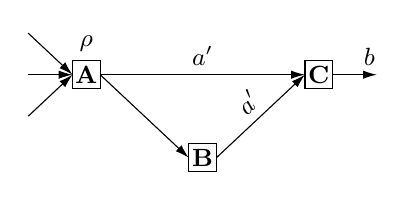
\begin{tikzpicture}[scale=1]
  
  \small
  
  \newcommand\X{210/5pt};
  \newcommand\Y{30pt};
  
  \draw[->] ( -0.5*\X, 0.5*\Y) -- ( -5+0*\X, 0*\Y);
  \draw[->] ( -0.5*\X, 0*\Y) -- ( -5+0*\X, 0*\Y);
  \draw[->] ( -0.5*\X, -0.5*\Y) -- ( -5+0*\X, 0*\Y);  

  \draw[fill=white] (0*\X, 0*\Y) node{\textbf{A}} +(-5pt, -5pt) rectangle +(5pt, 5pt);
  \draw (0*\X, 5-0*\Y) node[anchor=south]{$\rho$};
  \draw[fill=white] (1*\X, -1*\Y) node{\textbf{B}} +(-5pt, -5pt) rectangle +(5pt, 5pt);
  \draw[fill=white] (2*\X,  0*\Y) node{\textbf{C}} +(-5pt, -5pt) rectangle +(5pt, 5pt);

  \draw[->](5+0*\X, 0*\Y) -- (-5+1*\X, -1*\Y); %% A->B
  \draw[->](5+1*\X, -1*\Y) -- node[sloped, above]{$a'$} (-5+2*\X, 0*\Y); %% B->D
  
  \draw[->] (5+0*\X, 0*\Y)  -- node[anchor=south]{$a'$} (-5+2*\X, 0*\Y); %% A->B

  \draw[->](5+2*\X, 0*\Y) -- node[anchor=south west]{$b$}( 2.5*\X, 0*\Y);
\end{tikzpicture}}
    \caption{\label{fig:preventivesolve}Preventive causal broadcast does not violate
      causal order in dynamic networks anymore.}
  \end{center}
\end{figure*}

Algorithm~\ref{algo:bufferbroadcast} shows the instructions of our preventive
causal broadcast. Its two operations broadcast and deliver rely on reliable
broadcast (see Algorithm~\ref{algo:reliablebroadcast}). In fact, without
additions nor removals of links, our protocol only executes instructions of
reliable broadcast (see Line~\ref{line:rbroadcast},~\ref{line:rdeliver}).

\begin{theorem}[\CBROADCAST is causal in static networks\label{theo:static}]
  \CBROADCAST is a causal broadcast in static networks.
\end{theorem}

\begin{proof}
  In static networks, \CBROADCAST only executes the instructions of reliable
  broadcast. Reliable broadcast along with FIFO links ensures causal broadcast.
  The proof can be found in Paper~\cite{friedman2004causal}.
\end{proof}

The removal of links and the departure of processes are not an issue, for it
does not reorder messages traveling through the links\footnote{It may create
  partitions infringing the uniform agreement property. Network partitioning
  constitutes an orthogonal problem that we do not address in this
  paper.}. Algorithm~\ref{algo:bufferbroadcast} does not provide specific
instructions for such cases.
% However, it may create partitions. It is an orthogonal problem

\begin{lemma}[\CBROADCAST is causal in dynamic networks subject to
  removals\label{lem:removals}]
  \CBROADCAST is a causal broadcast in dynamic networks where processes can
  leave the network or links can be removed.
\end{lemma}

\begin{proof}
  Removing a process from the network and removing all the incoming and outgoing
  links of this process is equivalent. We assume that removals do not create
  network partitions.  Removing a link does not change the delivery order of
  causally related messages. Identically to the proof of
  Theorem~\ref{theo:static}, our causal broadcast only executes instructions of
  reliable broadcast in such cases. The proof is identical to that of
  Paper~\cite{friedman2004causal}.
\end{proof}

Our causal broadcast becomes more sophisticated when the process adds links.
Figure~\ref{fig:preventiveproblem} shows the issue with link additions.  New
links may act as shortcut for messages. First messages that travel through new
links may arrive before preceding messages that took longer paths. New links
create additional diffusion paths that potentially disorder messages.  Solving
this issue requires that even new links convey all messages in the right
order. Sending all broadcast messages since the beginning would be too
costly. Instead, a process $p$ creating a link to a process $q$ needs to know
the messages received by $q$ to send potentially missing messages in the right
order using this link. While obtaining $q$'s acknowledgment would be costly in
general settings, using already created FIFO links keeps it cheap. Once missing
messages have been sent through this new link, $p$ starts to use it
normally. New links do not create diffusion paths that could break causal order.

Compared to reliable broadcast, Algorithm~\ref{algo:bufferbroadcast} adds a
structure associating each new link with a buffer of
messages. Figure~\ref{fig:preventivesolve} shows how it solves causal order
violations. In Figure~\ref{fig:preventivesolveA}, Process~A broadcasts $a$.  In
Figure~\ref{fig:preventivesolveB}, it wants to add a link to Process~D. It sends
a locked message $\ell$ to process~D (see Line~\ref{line:sendlocked}) and awaits
for the later's acknowledgment.  We leave aside the implementation of this send
function (e.g. broadcast or routing). Although, using already established FIFO
links constitutes a cheap way to achieve it. While awaiting, Process~A keeps its
normal functioning and maintain a buffer of messages associated with the new
link (see Line~\ref{line:bufferbroadcast},~\ref{line:bufferforward}). In
Figure~\ref{fig:preventivesolveC}, Process~A broadcasts another message $a'$. It
sends it normally to Process~B but does not send it to Process~D
directly. Instead, it buffers it. In Figure~\ref{fig:preventivesolveD},
Process~D receives Process~A's locked message $\ell$. Since links are FIFO, it
implicitly means that Process~D also received $a$. Process~D sends an
acknowledgment $\alpha$ to Process~A (see Line~\ref{line:sendack}). $\alpha$ can
travel through any communication mean. In Figure~\ref{fig:preventivesolveE},
Process~A receives $\alpha$. Consequently, Process~A knows that Process~D
received and delivered at least $a$ and all preceding messages. It empties the
buffer of messages to Process~D (see Line~\ref{line:emptybuffer}). Afterwards,
Process~A uses the new link normally.

The acknowledgment phase ensures that Process~D received all messages preceding
$a$ and $a$ itself. The buffering phase ensures that Process~D receives all
messages between the sending of the locked message $\ell$ and the receipt of
Process~D's acknowledgment $\alpha$. Afterwards, Process~D will receive
Process~A's broadcast or forwarded messages from this new direct link or
transitively through Process~B.

\begin{lemma}[\CBROADCAST is causal in dynamic networks subject to
  additions\label{lem:additions}]
  \CBROADCAST is a causal broadcast in dynamic networks where processes can join
  the network or links can be added.
\end{lemma}

\begin{proof}
  To prove that \CBROADCAST is a causal broadcast, we must show that it ensures
  validity, uniform agreement, uniform integrity, and causal order -- that is
  FIFO order and local order. \\
  \textbf{Validity, uniform agreement, uniform integrity:} \CBROADCAST is an
  \textsc{R-broadcast}. \\
  \textbf{FIFO:} Suppose a process $p$ broadcasts $m$ before $m'$. Consider that
  a correct process $q$ delivers $m'$. We must show that $q$ delivers $m$ before
  $m'$.  Since adding a FIFO link from a Process $r$ to any other Process $s$ is
  like adding potential FIFO paths from $p$ to $q$, we summarize this as a link
  from $p$ to $q$ with arbitrary settings but still FIFO.  \TODO{Should this be
    a proof?  Maybe a proof of equivalent model if kept}. \\
  Since Process $q$ delivers $m'$ it either received $m'$ from already well
  established links, or from the new one. In the former case, the proof is
  identical to that of Theorem~\ref{theo:static}. In the latter case, Process
  $q$ delivers $m'$ means that Process $p$ broadcasts $m$ then $m'$ either
  \begin{inparaenum}[(i)]
  \item \label{case:one} $m'$ during buffering and $m$ before buffering;
  \item \label{case:two} $m'$ during buffering and $m$ during buffering;
  \item \label{case:three} $m'$ after acknowledgment and $m$ before buffering;
  \item \label{case:four} $m'$ after acknowledgment and $m$ during buffering;
  \item \label{case:five} $m'$ after acknowledgment and $m$ after acknowledgment.
  \end{inparaenum}
  We must show that either 
  \begin{inparaenum}[(1)]
  \item \label{show:one} Process $q$ already received $m$ from another link
    before receiving $m'$ from the new link,
  \item \label{show:two} or that this new link conveyed $m$ before $m'$.
  \end{inparaenum}

  \begin{itemize}
  \item [(\ref{case:one})] Process $p$ put $m'$ in the buffer. Process $p$
    empties the buffer containing $m'$ after $p$ received an acknowledgment
    meaning that at least $m$ has been received at $q$. This
    shows~(\ref{show:one}).
  \item [(\ref{case:two})] Process $p$ put $m$ then $m'$ in the buffer. When the
    acknowledgment is received, it sends $m$ then $m'$ to Process $q$. This
    shows~(\ref{show:two}).
  \item [(\ref{case:three})] Identical to case~(\ref{case:one}) without the need
    of buffering.
  \item [(\ref{case:four})] Since Process $p$ empties the buffer containing $m$
    when it receives the acknowledgment, and since Process $p$ broadcasts $m'$
    afterwards using the new link, it shows~(\ref{show:two}).
  \item [(\ref{case:five})] It directly shows~(\ref{show:two}).
  \end{itemize}
  %%%%%%%%%%%%%%%%%%%%%%%%%%%%%%%%%%%%%%%%%%%%%%%%%%%%%%%%%%%%%%
  % If Process $p$ broadcasts $m$ before the link addition, Process $p$ either
  % broadcasts $m'$ during buffering phase or after acknowledgment: 
  % \begin{itemize}
  % \item In the former case, since the receipt of $m$ precedes the creation of the
  %   acknowledgement, when $p$ receives the acknowledgement, it empties the buffer
  %   containing $m'$ to $q$. Hence, from any path, Process $q$ receives and
  %   delivers $m$ before $m'$.
  % \item In the later case, the acknowledgement confirms that $q$ received
  %   $m$. Afterwards, when $p$ broadcasts $m'$ it travels, among others, the newly
  %   created link, and eventually arrives to $q$.
  % \end{itemize}
  %%%%%%%%%%%%%%%%%%%%%%%%%%%%%%%%%%%%%%%%%%%%%%%%%%%%%%%%%%%%%%%
  % If Process $p$ broadcasts $m$ during buffering phase, Process $p$ either
  % broadcasts $m'$ during buffering phase or after acknowledgement.
  % \begin{itemize}
  % \item In the former case, $p$ puts $m$ in the buffer before $m'$. When $q$
  %   receives $m'$, either it already received $m$ from another FIFO channel or
  %   it already received $m$ from the emptied buffer that contained $m$ before
  %   $m'$.
  % \item In the later case, When $q$ receives $m'$, either it received $m$ from
  %   FIFO channel or the buffer that empties after acknowledgment.
  % \end{itemize}
  %%%%%%%%%%%%%%%%%%%%%%%%%%%%%%%%%%%%%%%%%%%%%%%%%%%%%%%%%%%%%%%
  % If Process $p$ broadcasts $m$ after acknowledgement, Process $p$ broadcasts
  % $m'$ after acknowledgement. It corresponds to the static network (see proof of
  % Theorem~\ref{theo:static}).
  % In any case, process $q$ delivers $m$ before $m'$. \\
  \textbf{Local:} Since broadcast and forward have identical instructions, the
  proof is identical to that of FIFO order. \\
  % Suppose a process $p$ delivers $m$ before broadcasting $m'$. Consider a
  % correct process $q$ that delivers $m'$. We must show that $q$ delivers $m$
  % before $m'$. Just as the proof for Theorem~\ref{theo:static}, the difference
  % in our Algorithm compared to FIFO order demonstration is that Process $q$ may
  % have already received -- or is the origin of the broadcast of --
  % $m$. \TODO{Not over}  
  \textbf{Causal:} From Theorem~\ref{theo:causal}, since \CBROADCAST ensures
  both FIFO order and local order, it ensures causal order.
\end{proof}

\begin{theorem}[\CBROADCAST is a causal broadcast]
  \CBROADCAST is a causal broadcast in both static and dynamic network settings.
\end{theorem}

\begin{proof}
  For static networks, it comes from Theorem~\ref{theo:static}. For dynamic
  networks, it comes from Lemmas~\ref{lem:removals}~and~\ref{lem:additions}.
\end{proof}

\begin{algorithm}
  
\SetKwProg{Function}{function}{}{}
\SetKwProg{Upon}{upon}{}{}
\SetKwProg{Initially}{INITIALLY:}{}{}
\SetKwProg{Dissemination}{DISSEMINATION:}{}{}
\SetKwProg{Buffer}{BOUNDING BUFFERS:}{}{}
\SetKwProg{Failure}{HANDLING FAILURES:}{}{}

\small

\DontPrintSemicolon
\LinesNumbered

\Initially {} {
  % $Q$ \tcp*{$p$'s neighborhood, FIFO channels}
  $B$ \tcp*{link $\rightarrow$ buffered messages}
  \BlankLine
  $I \leftarrow \varnothing$ \tcp*{message id $\leftrightarrow$ link}
  $R \leftarrow \varnothing$ \tcp*{link $\rightarrow$ number of retries}
  \BlankLine
  $maxSize \leftarrow \infty $ \;
  $maxRetry \leftarrow \infty$ \;
}

\BlankLine

\Buffer {} {

  \Upon{\textsc{sendLocked}($from,\, to,\, id$)}{
    \lIf{$q \not\in R$} {$R[q] \leftarrow 0$}
    $I[id] \leftarrow to$ \;
  }

  \BlankLine
  
  \Upon{\textsc{receiveAck}($from,\, to,\, id$)}{
    $I \leftarrow I \setminus id$ \;
    $R \leftarrow R \setminus to$ \;
  }
  
  \BlankLine

  \Upon{\textsc{FBC-deliver$^+$}($m$)} {
    \ForEach{$q \in B$ \textbf{\textsc{such that}} $|B[q]| > maxSize$
      \label{line:maxsize}}{
      $\textsc{retry}(q)$ \;
    }
  }

  \BlankLine

  \Upon{\textsc{close}($q$)} {
    \lFor{$i \in I$ \textbf{\textsc{such that}} $I[i]=q$}{$I \leftarrow I \setminus i$}
    $R \leftarrow R \setminus q$ \;    
  }

  \BlankLine

  \Function{\textsc{retry}($q$)}{
    \lFor{$i \in I$ \textbf{\textsc{such that}} $I[i]=q$}{$I \leftarrow I \setminus i$}
    
    \If{$q \in R$} {
      $R[q] \leftarrow R[q]+ 1$ \;
      \lIf{$R[q] \leq maxRetry$} {\textsc{open}($q$)}
      \lElse{\textsc{close}($q$)}    
    }
  }
}  

\BlankLine

\Failure {} {

  \Upon{\textsc{timeout}($from,\, to,\, id$)}{
    \lIf {$id \in I$} {\textsc{retry}($to$)\label{line:timeout}}
  }

}


%%% Local Variables:
%%% mode: latex
%%% TeX-master: "../paper"
%%% End:

  \caption{\label{algo:boundingbuffer}Bounding the size of buffers and handling
    network failures.}
\end{algorithm}

While Algorithm~\ref{algo:bufferbroadcast} ensures causal order of message
deliveries, buffers consume unbounded space. For instance, if the message
acknowledging the locked message fails to reach its destination, the
corresponding buffer continues to grow over broadcast and forwarded messages. 

Algorithm~\ref{algo:boundingbuffer} aims to bound the size of buffers and handle
network failures, i.e., crashed processes or lost messages. Now, our causal
broadcast can reset the buffer of a new link. Resets happen when either the
buffer size is above a threshold (see Line~\ref{line:maxsize}), or the
acknowledgment message took too long to come back (see
Line~\ref{line:timeout}). Each locked message has an identifier corresponding to
a link. When a process receives an acknowledgment, it knows if it expired due to
a timeout. We only keep the buffer corresponding to the latest locked
message. We bound the number of retries so the protocol does not stay stuck in a
loop of retries.

\TODO{Example of failure management? (Will not look nice).}

% \begin{algorithm}
%   \SetKwProg{Function}{function}{}{}
\SetKwProg{Upon}{upon}{}{}
\SetKwProg{Initially}{INITIALLY:}{}{}
\SetKwProg{Communication}{COMMUNICATION:}{}{}
\SetKwProg{Buffer}{BOUNDING BUFFERS:}{}{}
\SetKwProg{Failure}{HANDLING FAILURES:}{}{}

\small

\DontPrintSemicolon
\LinesNumbered

\Initially {} { 
  $Q$ \;
}

\BlankLine

\Communication {} {
  
  \Function{\textsc{sendLocked}($from,\, to,\, id$) } {
    \lForEach {$q \in Q$} 
    {\textsc{sendTo}($q,\, \langle 'fwd',\, from,\, to,\, id \rangle$)}
  }

  \BlankLine
  
  \Upon{\textsc{receivedFwd}($from,\, to,\, id$)} {
    \lIf {$to \in Q$} {\textsc{sendTo}($to,\, \rangle 'locked',\, from,\, to$ }
  }
  
}

%%% Local Variables:
%%% mode: latex
%%% TeX-master: "../paper"
%%% End:

%   \caption{\label{algo:sendfunctions}Implementation of sending functions in
%     neighbor-to-neighbor peer-sampling protocols.}
% \end{algorithm}


%% \subsection{Proofs}

%% This section provides the proofs that our approach work in both static and
%% dynamic networks.



\subsection{Complexity}
\label{subsec:complexity}

We review and discuss about the complexity of \CBROADCAST. We distinguish the
complexity of causal ordering, the complexity of reliable broadcast, and the
complexity brought by the overlay network.

\PAR{Causal ordering.}{Regarding traffic, broadcast messages do not need to
  convey any control information. However, processes must send each message to
  all their neighborhood exactly once. It creates as many copies as
  neighbors. This number of copies may constitute an issue when the size of
  messages is large. To solve this issue, processes can send identifiers instead
  of large messages then send these messages on demand.  It introduces
  additional delays in communications but greatly reduces generated traffic
  (\REF).  Regarding local space consumption, our protocol maintains one buffer
  per link during its acknowledgment time. We assume that this time is short so
  the number of buffered messages stays small. Network conditions can make this
  assumption false. Algorithm~\ref{algo:boundingbuffer} allows to bound the size
  of each buffer and handle network failures.}

% While Algorithm~\ref{algo:bufferbroadcast} shows no buffer management which
% means that they can grow unbounded, we can easily bound them. For instance,
% above a threshold we clear the buffer and send another locked message, or we
% remove the link altogether.

\PAR{Reliable broadcast.}{Algorithm~\ref{algo:reliablebroadcast} shows the
  instructions of reliable broadcast. Even in presence of message duplicates it
  avoids multiple deliveries of a same message. To achieve this, the most
  straightforward structure is a set saving all new received messages. However,
  it increases linearly with the number of delivered messages (\REF). Assigning
  a unique identifier $\langle p,\, counter \rangle$ to each message changes the
  complexity. It becomes a vector that increases linearly with the number of
  processes that ever broadcast a message~\cite{fidge1988timestamps}. Using
  interval tree clocks~\cite{almeida2008interval} slightly overloads messages
  with identifiers but it improves the space complexity: the local structure
  increases linearly with the number of processes that are currently involved in
  broadcasting.}


% \TODO{Rework.} Represented in Algorithms~\ref{algo:fifobroadcast}
% and~\ref{algo:bufferbroadcast} by Function $alreadyReceived$. Causal ordering
% and detecting duplicated receipts are orthogonal problems. In this paper, we do
% not provide an implementation for the later. The simplest approach consists in
% saving all received messages (\REF). However, the size of this set linearly and
% monotonically increases as the number of broadcast messages increases. One would
% prefer an approach based on vectors where one entry corresponds to the number of
% messages received by a particular process~\cite{fidge1988timestamps}. Such
% approach do not require to piggyback additional data in the message. However, it
% requires to store locally a vector the size of which increases linearly compared
% to the number of processes that ever broadcast a message. Interval tree
% clocks~\cite{almeida2008interval} allow processes to reduce this complexity. It
% becomes linear in terms of number of processes that are currently involved in
% broadcasting. Possible improvements could take advantage of the fact that the
% number of duplicates is equal to the number of incoming links. However, it does
% not hold in dynamic networks where additional links are established. Finding a
% sublinear bound for detecting duplicated receipts remains an open problem.


\PAR{Overlay network.}{Values such as the number of messages sent by each
  process, or the number of hops for a message to reach all processes, are
  interdependent values brought by the overlay network. For instance, random
  peer-sampling protocols~\cite{jelasity2007gossip} build network overlays with
  properties similar to those of random graphs~\cite{erdos1959random}. They
  provide each process with a random subset of neighbors the size of which is
  considerably smaller than the network size. Since the neighborhood size is
  logarithmic compared to the network size, the number of messages sent by each
  process for each broadcast message is logarithmic.  Since random peer-sampling
  protocols build topologies close to random graphs, messages take a logarithmic
  number of hops to reach all processes. In addition, random peer-sampling
  protocols such as \SPRAY~\cite{nedelec2017adaptive} or
  \CYCLON~\cite{voulgaris2005cyclon} create links using only
  neighbor-to-neighbor interactions, i.e., they establish links only two hops
  apart. It takes only 4 hops for a new link to get acknowledged.  The overhead
  brought by these messages is negligible. The acknowledgment time of buffers,
  hence the size of buffers, remains small.}

The next section reviews state-of-the-art techniques designed to maintain causal
order among messages.

%%% Local Variables:
%%% mode: latex
%%% TeX-master: "../paper"
%%% End:


\section{Related work}
\label{sec:relatedwork}

This section reviews the related work of logical clocks. It goes from
piggybacking approaches to vector approaches and their following compaction
approaches. Then, it reviews semantic dependency tracking and dissemination path
approaches.

\noindent \textbf{Piggybacking
  approaches~\cite{birman1987reliable,hadzilacos1993fault}}. A trivial way to
ensure causal ordering of messages is to piggyback all causally related messages
since the last broadcast message along with the new broadcast message. Even by
piggybacking the identifiers of messages instead of messages themselves, the
broadcast message size may increase quickly depending on the
application. \CBROADCAST does not piggyback all preceding messages in broadcast
messages. However, an accumulation of messages arises during buffering. As
discussed in Section~\ref{subsec:complexity}, we can assume that links quickly
become safe so the buffer size stays small, and we can easily set a threshold on
the buffer size (see Algorithm~\ref{algo:boundingbuffer}).

\noindent \textbf{Vector clock
  approaches~\cite{fidge1988timestamps,mattern1989virtual}.}  A vector clock is
a vector of monotonically increasing counters.  It encodes the partial order of
messages using this vector: $VC(m) < VC(m') \implies m \rightarrow m'$.  Before
delivering a message, processes using vector-based broadcast check if the vector
of the message is ready regarding their local vector. If it detects any missing
preceding message, the process delays the delivery.  To implement this
vector-based broadcast
\begin{inparaenum}[(i)]
\item each process must maintain a vector locally;
\item each message must piggyback such vector;
\item there is 1 counter for each process of the network.
\end{inparaenum}
To accurately track causality, processes cannot share their entry. To safely
track causality, processes cannot reclaim entries. Hence, even with
\textbf{compaction approaches~\cite{singhal1992efficient}}, the vectors grow
linearly in terms of number of processes that ever broadcast a message.
In~\cite{almeida2008interval}, the complexity is reduced to the actual number of
processes in the network.  Still, these approaches do not scale, particularly in
dynamic networks subject to churn and failures. \textbf{Probabilistic
  approaches~\cite{mostefaoui2017probabilistic}} sacrifices on causality
tracking accuracy: messages may be delivered out of order under a computable
boundary. The size of control information in messages
depends on the desired boundary. \\
In comparison to these vector-based approaches, our approach reduces the
generated traffic of causal broadcast by a factor of $N$ in the most common
context where processes have partial knowledge of the network membership.
% It alleviates messages from the need to piggyback heavy
  % control information~\cite{friedman2004causal}
Unlike vector-based approach, our broadcast cannot state if two messages are
concurrent, accurate causal delivery is a feature provided by default by the
propagation scheme. Once a safe FIFO link is established, it delivers message in
the causal order with no delay at the speed of the FIFO link.


\noindent Explicitly tracking \textbf{semantic dependencies} allows broadcast
protocols to reduce the size of piggybacked control
information~\cite{bailis2013bolton,lloyd2011cops,mukund2014optimized}. For
instance, when Alice comments Bob's picture, everyone must receive the picture
before the comment. The broadcast message only conveys one semantic
dependency. When Alice comments multiple pictures at once, the broadcast message
conveys all dependencies.  Message overhead increases linearly with the number
of semantic dependencies. To track semantic dependencies, causal broadcast
becomes application dependent. Instead our approach remains
application-agnostic. Comments, pictures, etc. are events that relate to all
preceding events. When Alice comments Bob's picture, everyone will receive this
event before the former event and all other preceding events. Whatever the
number of preceding events, broadcast messages only convey constant size control
information.

\noindent Preserving causal order using \textbf{dissemination paths} reduces
generated traffic by keeping message overhead
constant~\cite{bravo2017saturn,friedman2004causal}. State-of-the-art does not
support dynamic systems~\cite{friedman2004causal}, or supports it using
epochs~\cite{bravo2017saturn} that confines usability to small scale systems
where failures are uncommon. In comparison, we designed \CBROADCAST to handle
large and dynamic systems. Our approach provides a lightweight and efficient
mean to reconfigure dissemination paths using local knowledge without impairing
causal order.  Saturn~\cite{bravo2017saturn} along with \CBROADCAST could ease
the former's online changes in configuration.


% \PAR{Topological approaches.}{A trivial way to ensure causal delivery of
% messages without message overhead consists in building an overlay network shaped
% as a ring: each broadcast message loops once in FIFO order (\REF).
% Unfortunately, maintaining a specific topology can prove costly in dynamic
% networks subject to churn. Our approach relies on a peer-sampling protocol
% \TODO{(Relies on R-broadcast that relies on such psp)} but we make no assumption
% on the built topology. One can choose the most suitable topology depending on
% network settings. For instance, random peer-sampling
% protocols~\cite{jelasity2007gossip} have a low upkeep and guarantee a connected
% network even in dynamic settings.}

% \TODO{Explain super-peer approaches.}

% \TODO{Inter-group broadcast is a kind of topological approach.}

% \PAR{Inter-group
%   broadcast~\cite{johnson1998scalable,johnson1999intergroup}.}{Inter-group
% broadcast allows processes to broadcast messages to members of several
% inter-connected networks. Paper~\cite{johnson1999intergroup} states that
% inter-group causal broadcast is ensured when groups that internally ensure
% causal broadcast are linked together by communication channels that ensure FIFO
% ordering of messages. One can employ these approaches to cluster the network in
% subsystems. Control information in messages depends of the size of each small
% subsystem. Our approach is an extreme case where each process is a
% subsystem.}

%% The union of paths taken by broadcast messages builds a diffusion tree, i.e.,
%% a directed acyclic graph, that may change at each broadcast.

% \paragraph{Push-pull~\cite{mercier2017optimal}.} In random graphs, pull is
% optimally fast. Push phase of push-pull improves the startup phase of message
% dissemination. We only present push but it easily can be push-pull. \TODO{Maybe
%   too linked to random graphs.}


%%% Local Variables:
%%% mode: latex
%%% TeX-master: "../paper"
%%% End:


\section{Conclusion}
\label{sec:conclusion}

In this paper, we described a non-blocking causal broadcast protocol that breaks
scalability barriers for large and dynamic systems. Using \CBROADCAST, message
overhead and delivery execution time remain constant.
% Its space complexity remains small and can be bounded easily. 
Causal broadcast finally becomes an affordable and efficient middleware for
large scale distributed applications running in dynamic environments.

As future work, we plan to investigate on reducing the space complexity of
reliable broadcast. Section~\ref{subsec:complexity} reviews structures with
linearly increasing space consumption. We can reduce this complexity in static
systems. We can prune the structure from already received messages, for we know
that the number of duplicates is equal to the number of incoming
links~\cite{raynal2013distributed}. Unfortunately, this does not hold in dynamic
systems. We would like to investigate on a way to prune the structure in such
settings. This would make causal broadcast scalable as well on generated traffic
as on space consumption.

We also plan to investigate on retrieving partial order of
events. Section~\ref{sec:relatedwork} states that vector-based approaches allows
to compare an event with any other event. They can decide on whether one
precedes the other, or they are concurrent. They can build the partial order of
event using this knowledge. Our approach cannot by default. However, in extreme
settings where the overlay network is fully connected, we can assign a vector to
each received message using local knowledge only, and without message
overhead. We would like to investigate on a way to build these vectors locally
in more realistic settings where processes have partial knowledge of the
membership. % We would like to analyze its minimal cost.

%%% Local Variables:
%%% mode: latex
%%% TeX-master: "../paper"
%%% End:


% 
\section*{Acknowledgments}

This work was partially
funded by
% the French ANR project SocioPlug (ANR-13-INFR-0003), and by
% the DeSceNt project granted by the Labex CominLabs excellence laboratory
% (ANR-10-LABX-07-01).
the French ANR projects O'Browser (\mbox{ANR-16-CE25-0005-01}), and Descartes
(\mbox{ANR-16-CE40-0023}).

% Experiments presented in this paper were carried out using the Grid'5000
% testbed, supported by a scientific interest group hosted by Inria and including
% CNRS, RENATER and several Universities as well as other organizations (see
% \url{https://www.grid5000.fr}).

%%% Local Variables:
%%% mode: latex
%%% TeX-master: "../paper"
%%% End:


%%\bibliographystyle{abbrv}
\bibliography{bibliographie}
  
\end{document}

